\subsection{The monitoring}
\label{sec:monitoring}

The idea of a monitoring started with the necessity to make a report of the status of WebDAV/https over the grid. We needed to know which are the sites that are working fine with Davix, and have some details of the problem for those where data remote access was not working. Inicially, this report was generated in pdf, this is still the case but finally it could be provided at webpage:\\
\url{http://sblunier.web.cern.ch/sblunier/webdavGridStatus/}\\

This monitoring is updated every day.

\subsubsection{Structure of the monitoring}
The monitoring is divided in three parts:\\

\indent	\textbf{A. \underline{Local tests:}} two tests per sites are done on lxplus: first with curl and second with davix.\\
Before giving the results of the tests some more informations are given: the type of storage the version of the tested site, the file that will be tested and the date and hour of the tests.\\
The curl command is trying to reach the file, rucio redirects the url on the headnode of the site and the site is in charge to locate the file on the right disk. This is what is done on this test, if the file is not found the relevant error of curl is reported.\\
The second test try to open and read one branch of this file using Davix and reports if this could be done successfully.\\
All of those tests are used to create the plots thta appear in introduction that give more general statistics. First, there are two pie charts that give the proportions of tests that worked fine and the proportion per error and finally a plot giving the number of sites that where successfull per day.\\

\indent	\textbf{B. \underline{The WebDAV events rate:}} Compilation of the results that ran over the grid.\\
Each day, one job is sent on each ATLAS site that has a Datadisk. This job creates a list of one file per Datadisk of the same cloud. A routine is sent for each file that opens the file, read one branch measure the time needed to complete the reading part and sent this time in an Histogram. This operation is repeated 100 times, and creates one histogram per Datadisk of the cloud. This means that each histogram should contain 100 entries. That's not always the case since sometimes no file is found, if the file is found but could not be opened or read the bin 0 is incremented. All the histograms are saved in a root file and this file is the output of the job.\\

Those jobs are in fact sent three times with three different configuration:
	\begin{itemize}
		\item \textbf{configuration 1:} Davix access, TTreeCache disabled
		\item \textbf{configuration 2:} Davix access, TTreeCache enabled
		\item \textbf{configuration 3:} xrootd access, TTreeCache enabled
	\end{itemize}

We download the results about 18 hours before sending it. In this part there are 7 histograms. The first three histograms give the number of file that could be read for each jobs configuration. In fact this corresponds to the number of all entries of the histograms from the outputs that are different from zero. A column corresponds to the output of one job, each cell to one histogram from the outputs. The histograms 4, 5 and 6 give the mean of the time of events rate for each Datadisk and the error.
The last histogram makes a direct comparison between the histograms 5 and 6: it represend the ratio (Davix events rate)/(xrootd event rates). If the result is above one Davix access is faster if not xrootd is faster.\\

\indent	\textbf{C. \underline{The jobs on the queues:}} Statistics about the jobs that ran for the previous part.\\
This part gives the status of the jobs for each configuration after the tests. Three status are possible: done (the job complete successfully), running (the job is running or has not been started), failed (crash of the job). A pie chart compile the proportion per status of the jobs.

\subsubsection{Technical details}

In this part we will explain in details how the monitoring is generated. The inicial idea of all of this work was only to make the first part in a pdf and became gradually bigger, it was not thought to give the other part so the code might not be easy to read. Nevertheless, at the end some effort was done to make it more ergonomic for the developer and hopefully can be read, maintained and even improved by some else. \\

The different languages used for this monitoring are C++, python, bash script, latex and html, however no html knowing is needed to purchase this work because it is directly generated by compiling latex. \\

The main folder is \textit{WebDAVMonitor} it contains 4 folders has shown in figure \ref{fig:WebDAVMonitor}. We will detail all of those parts.\\

\begin{figure}
	\center
	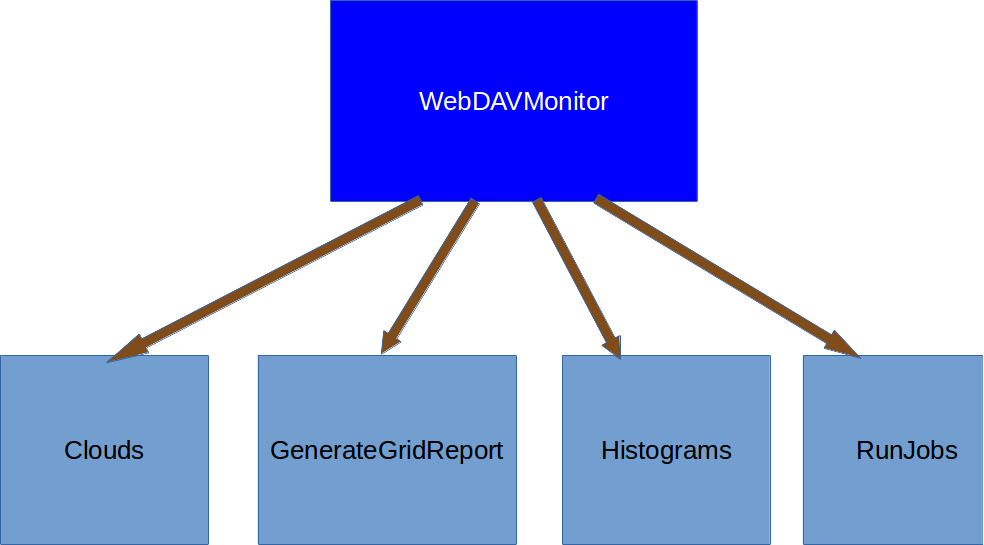
\includegraphics[width=0.7\textwidth]{WebDAVMonitor}
	\caption{Structure of WebDAVMonitor}
	\label{fig:WebDAVMonitor}
\end{figure}

\indent \textbf{A. \underline{Clouds:}}\\

\begin{figure}
	\center
	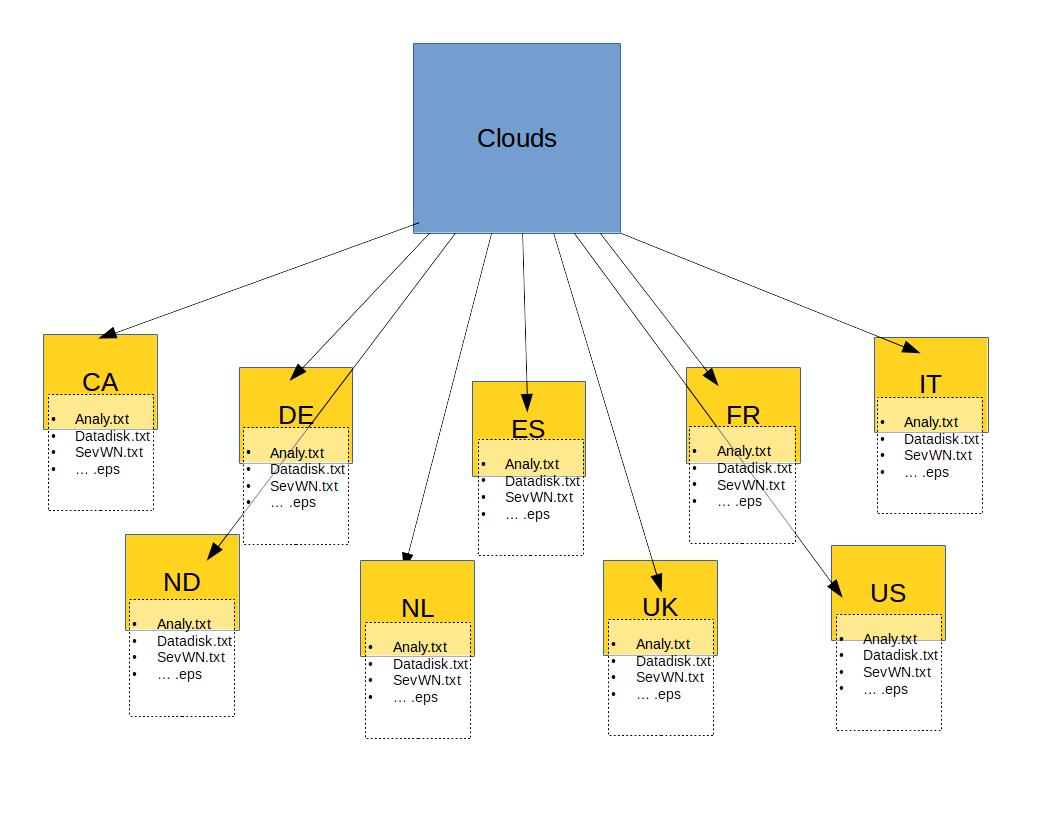
\includegraphics[width=0.8\textwidth]{Clouds}
	\caption{Structure of Clouds}
	\label{fig:Clouds}
\end{figure}

The folder \textit{Clouds} contains one folder per cloud, and each folder contains three files essential to the working of the monitoring:
\begin{itemize}
	\item \textit{Analy.txt:} contains the list of all the queues where we want to run the job on the cloud. This file will be read several times by the bash scripts that we will see later.
	\item \textit{Datadisk.txt:} like for the previous one, this file contains all Datadisks of the cloud, it's an exhaustive list.
	\item \textit{SEvsWN.txt:} to make the link between the disk and the queue that belong to the same cloud, will be used for the creation of matrix in part B of the monitoring.
\end{itemize}

The other files in those folder are file that are modified at each generation of the monitoring, they can be removed because they are not essential since they are created by the scripts:

\begin{itemize}
	\item \textit{PerCentFile.eps:} Histogram 1 of the monitoring, percent of file that could be read with configuration 1.
	\item \textit{tPerCentFile.eps:} Histogram 2 of the monitoring, percent of file that could be read with configuration 2.
	\item \textit{xPerCentFile.eps:} Histogram 3 of the monitoring, percent of file that could be read with configuration 3.
	\item \textit{EventRate.eps:} Histogram 4 of the monitoring, events rate with configuration 1.
	\item \textit{tEventRate.eps:} Histogram 5 of the monitoring, events rate with configuration 2.
	\item \textit{xEventRate.eps:} Histogram 6 of the monitoring, events rate with configuration 3.
	\item \textit{xRatio.eps:} Histogram 7 of the monitoring, ratio of common part of histogram 5 and 6.
	\item \textit{prun.txt:} prun commands that ran for the corresponding cloud, all the jobs are listed here, when a job is sent one line is written in this file. It's just an information file.
\end{itemize}

All the \textit{.eps} files are used to generate the monitoring, in fact when generating the latex the images are referenced directly in those folder.\\

\indent \textbf{B. \underline{RunJobs:}}\\

The rule of this folder is to send the jobs. It only contains files and this time most of them are essential. The general idea is to send one job per queue that will read 100 times one file per Datadisk of the cloud just as explained in the previous part. The jobs are labeled by a name of the type:
\begin{center}
	\textit{user.sblunier.?1allgrid????2.??3.ANALY\_?4}\\
\end{center}
where:
\begin{itemize}
	\item ?1 = m,t or x depending of the jobs configuration
	\item ????2 = number of the job, is incremented each day
	\item ??3 = name of the cloud
	\item ANALY\_?4 = site where the job is running
\end{itemize}
By doing that we guarantee that each job will have a different name (unless we reach ????2=9999)\\

\noindent \textbf{\textit{- main.C:}}
\textbf{Arguments:}\\
\begin{itemize}
	\item argv1: string, url of the file we are going to read
	\item argv2: string, name of the output file which will contain all the histograms.
	\item argv3: string, \textit{"ttreecache"} will activate TTreeCache while reading the file, something else disabled TTreeCache, there is no default argument
\end{itemize}

The output will be a file \textit{argv2.root} that contains the histograms. If the file exists the program will just append the bin to the histogram, else it creates it and append the measured value.\\

\noindent \textbf{\textit{- Makefile, main.o, main:}} For the compilation and executable of \textit{main.C}\\

\noindent \textbf{\textit{- listFilePeroSite.txt:}} Contains the list of file that will be read by \textit{main}. The url of the file is different depending on which protocol we want to use.\\
\noindent \textbf{\textit{- ttreeCacheBlackList.txt:}} When writing this report the root version used is 5.34.19-davix\_p1-x86\_64-slc6-gcc48-opt, with this version we get problems with some sites while using TTreeCache which make crash the jobs, this file contains the list of those sites. Nothing generates this file, it's purely based on testing the sites one by one.\\

\noindent \textbf{\textit{- launchJobs.sh:}} Read \textit{listFilePeroSite.txt:} and use it as argument to launch \textit{main} on each of the urls listed in.
\textbf{Arguments:}\\
\begin{itemize}
	\item arg1 = argv2 of main (\textit{ANALY\_SITE})
	\item arg2 = argv3 of main (\textit{"ttreecache"} or not)
\end{itemize}

If TTreeCache is enabled, the program checks if the site where the file is stored belongs to \textit{ttreeCacheBlackList.txt:}, if yes we look at the next one, else we process it normally.\\

\noindent \textbf{\textit{- getFiles.py:}} Python file that uses dq2 to pick some \textit{NTUP\_COMMON} files on the grid and store the url in \textit{- listFilePeroSite.txt:}. In the case of xrootd there is a list of endpoint corresponding to the site so that the file is able to create the url for xrootd. For WebDAV we use the general pattern of Rucio: \textit{"https://voatlasrucio-redirect-prod-01.cern.ch/redirect/"}.\\
\textbf{Arguments:}\\
\begin{itemize}
	\item sys.argv[1] = \textbf{"Davix"} or \textbf{"xrootd"} for the protocol needed
\end{itemize}

\noindent \textbf{\textit{- main.sh:}}

\textbf{Arguments:}\\
\begin{itemize}
	\item \$1: Cloud where the job is going to run
	\item \$2: argv2 of main (\textit{ANALY\_SITE})
	\item \$3: argv3 of main (\textit{"ttreecache"} or not)
	\item \$4: \textit{"davix"} or \textit{"xrootd"} depending on the protocol you want to use, argument necesarry to generate the right type of URL.
\end{itemize}

This script copies the file \textit{Datadisk.txt} in the local folder from the cloud corresponding to argument 2, run \textit{getFiles.py} using \textit{Datadisk.txt} and run \textit{launchJobs.sh}.\\

\noindent \textbf{\textit{- x509up\_u}xxxxx:} Valid proxy that will be needed for remote access, this file is sent with the job.\\

\noindent \textbf{\textit{- prun.txt:}} Output of the prun command executed by the script \textit{runPrun.sh}, information file.\\

\noindent \textbf{\textit{- runPrun.sh:}} The main function of this script is to execute the prun command to send the jobs. It also creates the files \textit{mjobIDs.txt}, \textit{tjobIDs.txt} and \textit{xjobIDs.txt} that will contain the number of the jobs by scanning the output of the prun command. This script activate the ATLAS commands (setupATLAS) activates Panda and dq2. It also select the root and Davix versions, copies the proxy from /tmp/.
It loops overall the folder of \textit{Clouds} and overall the items in \textit{Analy.txt} of the cloud, by doing that we send one job per queue giving the name of the output folder\\

\textbf{Arguments:}\\
\begin{itemize}
	\item \$1 = Cloud where you want the jobs to be sent, "all" for all the grid
	\item \$2 = number of the experiment, will be the number that labels the job serie (????2)
	\item \$3 = "ttreecache" or not
	\item \$4 = "davix" or "xrootd"
\end{itemize}

\begin{figure}
	\center
	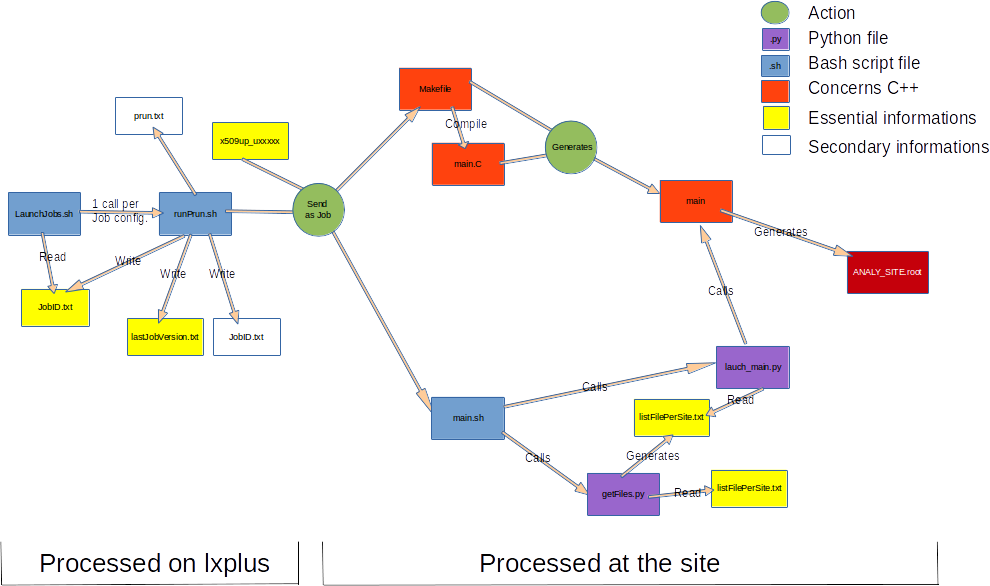
\includegraphics[width=1.1\textwidth]{runJobs}
	\caption{Block diagram of RunJobs}
	\label{fig:runJobs}
\end{figure}

Figure \ref{fig:runJobs} gives an overview of the working of all those files together.\\

\indent \textbf{C. \underline{Histograms:}}\\

The function of this folder is to contain the output of the jobs, meaning the \textit{.root} files.

\begin{figure}
	\center
	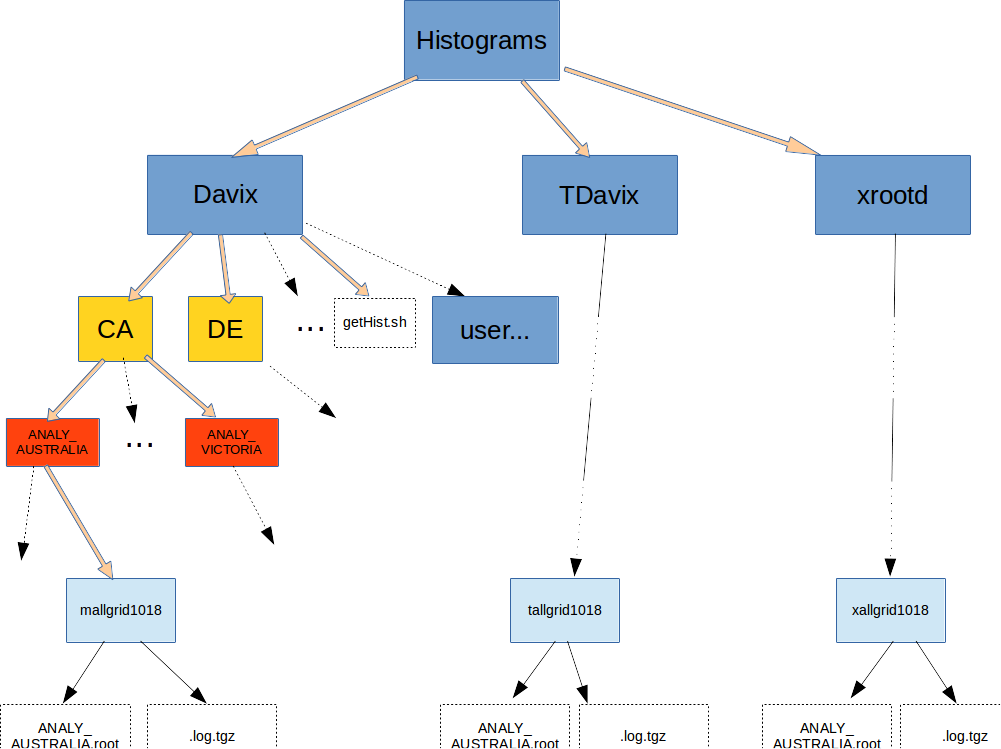
\includegraphics[width=0.7\textwidth]{histograms}
	\caption{Structure of Histograms folder}
	\label{fig:histograms}
\end{figure}

As shown in figure \ref{fig:histograms} the \textit{Histograms} folder contains three folders:

\begin{itemize}
	\item \textit{Davix}: Outputs of the first job configuration (TTreeCache disabled, Davix)
	\item \textit{TDavix}: Outputs of the second job configuration (TTreeCache enabled, Davix)
	\item \textit{xrootd}: Outputs of the third job configuration (TTreeCache enabled, xrootd)
\end{itemize}

They all have exactly the same structure, that's why we will only concentrate on the first one. The following depth contains folders named by the clouds, the clouds contains folders named by the queues where the jobs are ran. The queues folders contain folders that are called by the name of the corresponding experiment. This last folder is the one which will contain the outputs of the jobs: the \textit{.root} output and the logs.\\
This structure might be a little complicated but the goodness is that all the jobs are saved and we can at any moment have the details of a special result.\\
There might be others folder in \textit{Davix} that have the name of the jobs, they just are the outputs of the last downloaded job. \\

\indent \textit{\textbf{- getHist.sh:}} This script is here to distribute the outputs in their corresponding folders to keep them. It iterates over all the lines of the file \textit{clouds.txt} which is an essential file.\\


\indent \textbf{D. \underline{GenerateGridReport:}}\\

This part is the one which will write the latex report. It's divided in two sections, the first section treat all that requires dq2 and the second one generally needs root. This had to be separated because dq2 and root started to be incompatible during April 2014, this is not going to be fixed since dq2 is going to be replaced by Rucio.\\

Let us give an overview of those two parts before going into the details:

\begin{itemize}
	\item \textit{dq2Infos}: This part download and save the output of the jobs, generates one list of file url per cloud, and collect the versions of storage of the sites.
	\item \textit{writeLatex}: Generate the first part by testing curl and Davix locally, compile, creates, save the histograms and integrate them in the latex of part two and finally generate the part three by reading the html of the jobs on JEDI.
\end{itemize}


\begin{figure}
	\center
	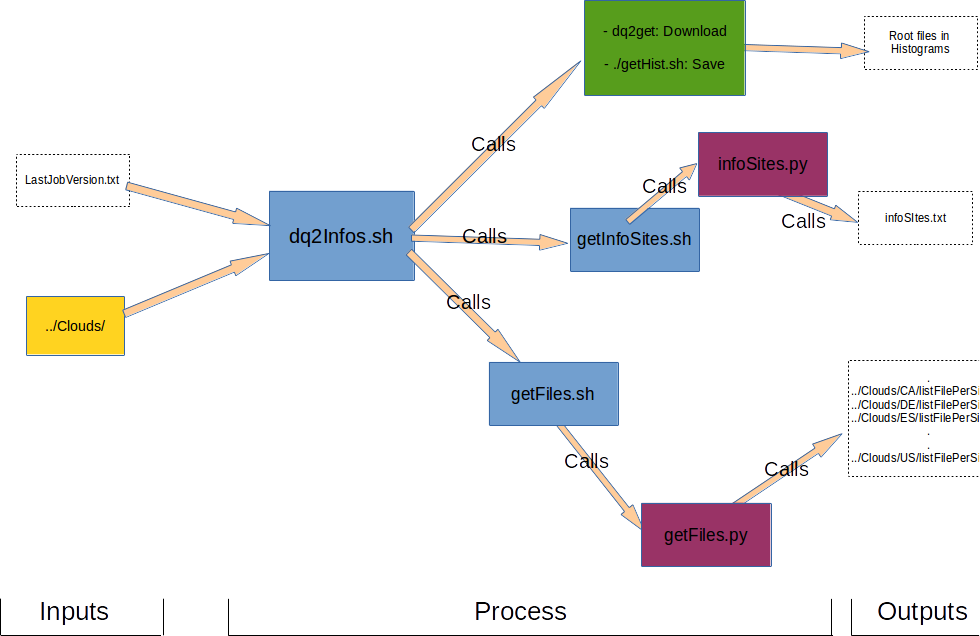
\includegraphics[width=0.9\textwidth]{dq2Infos}
	\caption{Functionning of \textit{dq2Infos.sh}}
	\label{fig:dq2Infos}
\end{figure}

In figure \ref{fig:dq2Infos} you can see how the first part is working, all the outputs will be necessary to produce the report with \textit{writeLatex.sh}, and in figure \ref{fig:writeLatex} the diagram for writeLatex which gives and overview on the last steps of the monitoring generation.


\begin{figure}
	\center
	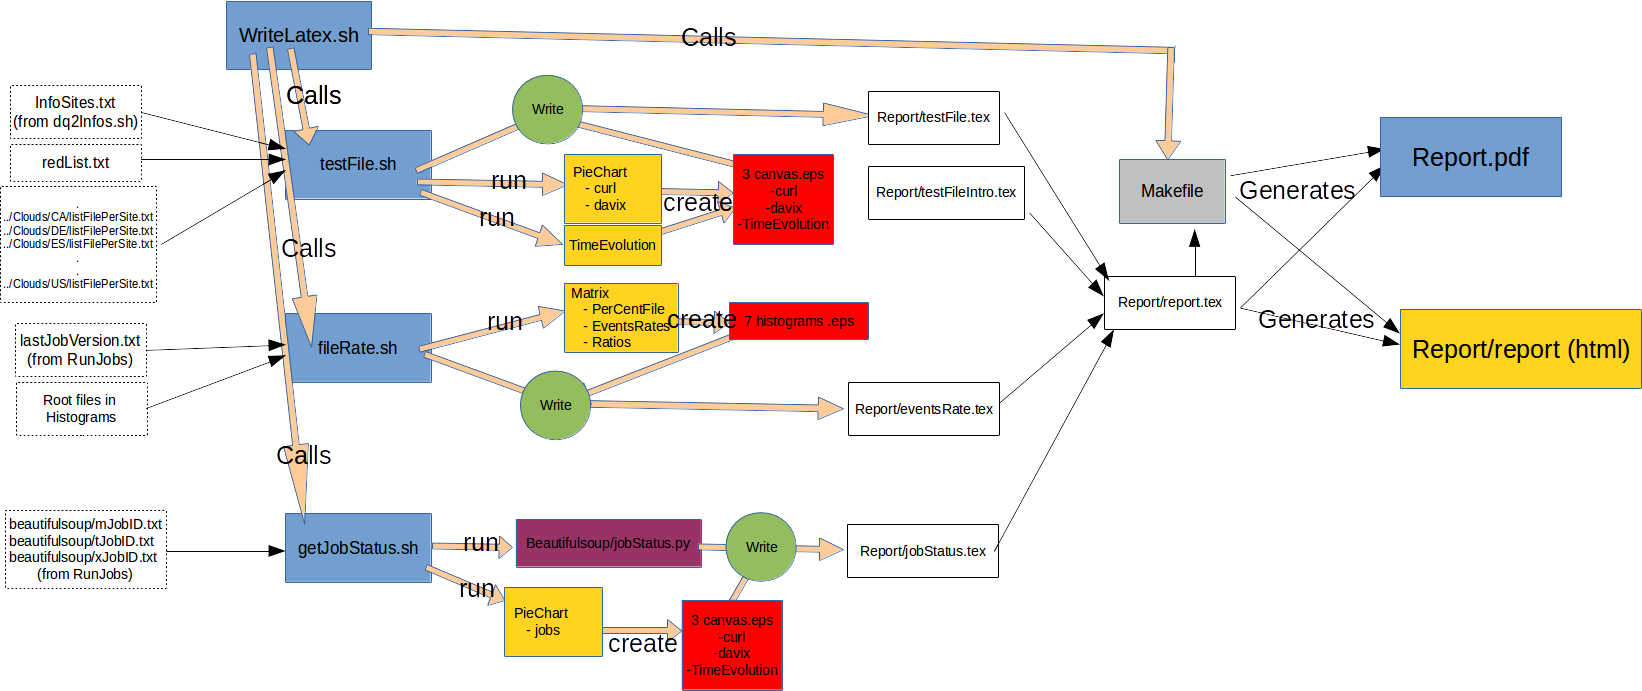
\includegraphics[width=1.1\textwidth]{writeLatex}
	\caption{Functionning of \textit{writeLatex.sh}}
	\label{fig:writeLatex}
\end{figure}
